\documentclass[conference]{IEEEtran}
\usepackage[spanish]{babel}
\usepackage{graphicx}
\usepackage{amsmath}
\usepackage{siunitx}
\usepackage{float}
\usepackage{placeins}
\usepackage{listings}
\usepackage{xcolor}
\usepackage[hidelinks]{hyperref}
\usepackage{grffile}

\lstset{
  basicstyle=\ttfamily\footnotesize,
  keywordstyle=\color{blue}\bfseries,
  commentstyle=\color{gray}\itshape,
  stringstyle=\color{teal},
  breaklines=true,
  frame=single,
  numbers=left,
  numberstyle=\tiny\color{gray},
  xleftmargin=1.5em,
  captionpos=b
}

% Placeholder visual para figuras aún no disponibles (no requiere archivo externo).
% Uso: \imgplaceholder{<alto>}{<descripcion de la imagen a insertar>}
\newcommand{\imgplaceholder}[2]{%
  \fbox{\begin{minipage}[c][#1][c]{\dimexpr\linewidth-2\fboxsep-2\fboxrule}%
    \centering\itshape\small #2
  \end{minipage}}%
}

\begin{document}

\title{Control por Retroalimentación de Estados de un Péndulo con Rueda de Reacción: Diseño de Controlador, Observador y Servosistema}

\author{
    \IEEEauthorblockN{
         García Araque Daniel, Nombre Estudiante 2, Nombre Estudiante 3
    }
    \IEEEauthorblockA{Ingeniería en Mecatrónica\\
    Universidad Militar Nueva Granada\\
    Cajicá, Colombia\\
  }
}

\maketitle

\begin{abstract}
Este informe presenta el diseño y la simulación de un sistema de control por retroalimentación de estados aplicado a un péndulo con rueda de reacción (rueda inercial), en el marco de la práctica de laboratorio de Tópicos Avanzados de Control. Se obtuvo el modelo en espacio de estados del sistema a partir de sus parámetros físicos, se determinaron sus representaciones en forma canónica controlable y observable, y se diseñaron controladores por ubicación de polos mediante tres metodologías equivalentes: asignación directa de coeficientes, compensación por matriz de pesos y el método de Ackermann. De igual forma, se diseñó un observador de estados diez veces más rápido que el controlador y un servosistema con compensador integrante para el seguimiento de referencias tipo escalón. Las simulaciones, ejecutadas en MATLAB a partir de las matrices reales del sistema, muestran la respuesta subamortiguada y críticamente amortiguada del lazo cerrado, la convergencia del error de estimación del observador y el seguimiento de referencia del servosistema.

\vspace{1em}
\noindent \textbf{\textit{Palabras clave---}} Espacio de estados, retroalimentación de estados, observador de Luenberger, servosistema, ubicación de polos, método de Ackermann, péndulo con rueda de reacción.
\end{abstract}

\section{Introducción}

Los métodos convencionales para el diseño de controladores, basados en el lugar geométrico de las raíces y en la respuesta en frecuencia, son útiles para sistemas de una entrada y una salida, ya que se fundamentan en la relación entrada-salida del sistema, es decir, en la función de transferencia o la respuesta al impulso \cite{ogata_discreto}. Estos métodos son conceptualmente sencillos y solo requieren de un número razonable de cálculos, pero su aplicabilidad se limita a sistemas lineales invariantes en el tiempo con una entrada y una salida; no se aplican a sistemas no lineales, salvo en casos simples donde la aproximación del comportamiento del sistema a una respuesta lineal es válida.

Los métodos convencionales tampoco son aplicables al diseño de sistemas de control óptimo y adaptable, que en su mayor parte son variantes en el tiempo y/o no lineales. Un sistema de control moderno puede tener muchas entradas y muchas salidas, interrelacionadas de manera compleja. Los métodos en el espacio de estado para el análisis y la síntesis de sistemas de control son más adecuados para tratar con sistemas con varias entradas y varias salidas que se requiere sean óptimos en algún sentido.

Este método se basa en la descripción del sistema en términos de $n$ ecuaciones diferenciales de primer orden, que pueden combinarse en una ecuación matricial diferencial de primer orden. La utilización de la notación matricial simplifica en gran medida la representación matemática de los sistemas de ecuaciones. El diseño en el espacio de estados se puede realizar para toda una clase de entradas, en lugar de una función de entrada específica, y permite incluir condiciones iniciales dentro del diseño, característica no contemplada en los métodos de diseño convencional \cite{ogata_discreto}.

El \textbf{estado} de un sistema dinámico es el conjunto más pequeño de variables (variables de estado) tales que el conocimiento de dichas variables en $t=t_0$, junto con el conocimiento de la entrada para $t\geq t_0$, determina por completo el comportamiento del sistema para cualquier $t \geq t_0$ \cite{ogata_discreto}. Si se necesitan $n$ variables para describir completamente el comportamiento de un sistema dado, estas $n$ variables se consideran las componentes de un \textbf{vector de estado} $\vec{x}$, y el espacio de $n$ dimensiones cuyos ejes coordenados están formados por $x_1, x_2, \dots, x_n$ se conoce como \textbf{espacio de estado} \cite{kuo_digital}. Las ecuaciones de estado están dadas por:

\begin{equation}
\dot{\vec{x}}(t) = A\vec{x}(t) + Bu(t)
\end{equation}
\begin{equation}
y(t) = C\vec{x}(t) + Du(t)
\end{equation}

La ley de control por retroalimentación de estados $u = -K\vec{x}$ modifica la matriz del sistema en lazo cerrado a $(A - BK)$, permitiendo ubicar arbitrariamente los polos del sistema siempre que el par $(A,B)$ sea controlable. Cuando no todos los estados $\vec{x}$ son medibles, se construye un \textbf{observador de estados} para estimarlos a partir de la salida medida $y(t) = C\vec{x}(t)$; la dinámica del error de estimación está gobernada por los polos de la matriz $(A - LC)$ \cite{unam_tutorial}. Finalmente, un \textbf{servosistema} es un sistema de control realimentado en el que la salida sigue una referencia de posición, velocidad o aceleración; su diseño incorpora un compensador integrante que aumenta en uno el orden del sistema para garantizar error de estado estacionario nulo ante entradas escalón.

En las siguientes secciones se presenta el modelo del péndulo con rueda de reacción utilizado en la práctica, sus representaciones canónicas, el diseño del controlador, del observador y del servosistema mediante las tres metodologías propuestas, y los resultados de las simulaciones obtenidas en MATLAB.

\section{Objetivos}

Reforzar los conceptos adquiridos del control en espacio de estados, incluyendo el uso de perturbaciones y observando el comportamiento de los controladores como filtros.

\subsection*{Objetivos Específicos}
\begin{itemize}
    \item Modelar el sistema mediante la representación en variables de estado bajo la forma canónica controlable y la forma canónica observable.
    \item Simular el sistema en espacio de estados usando MATLAB considerando perturbaciones.
    \item Controlar el sistema usando la ley de control $u=-K\vec{x}$.
    \item Diseñar observadores de estados.
    \item Diseñar servosistemas.
    \item Simular controladores por retroalimentación de estados e identificar su comportamiento como filtro.
\end{itemize}

\section{Marco Teórico}

\subsection*{Variables y espacio de estado}
Las variables de estado de un sistema dinámico conforman el conjunto más pequeño de variables que determinan su comportamiento completo: si se requieren al menos $n$ variables $x_1,x_2,\dots,x_n$ para que, dada la entrada para $t\geq t_0$ y el estado inicial en $t=t_0$, el estado futuro quede completamente determinado, dichas $n$ variables constituyen el conjunto de variables de estado \cite{ogata_discreto}. Estas variables no necesitan ser cantidades físicamente medibles; sin embargo, en la práctica es conveniente seleccionar cantidades fácilmente medibles.

\begin{figure}[H]
\centering
\imgplaceholder{5cm}{Espacio reservado -- Figura 1: Representación de estados de un sistema\\(diagrama de bloques $A(t)$, $B(t)$, $C(t)$, $D(t)$)}
\caption{Representación de estados de un sistema (diagrama de bloques $A(t)$, $B(t)$, $C(t)$, $D(t)$), reproducida de la guía de laboratorio \cite{unam_tutorial}.}
\label{fig:representacion_estados}
\end{figure}

\subsection*{Observadores de estado}
Cuando no se pueden medir todos los estados $\vec{x}$, se construye un observador para estimarlos, midiendo únicamente la salida $y(t)=C\vec{x}(t)$. El observador es básicamente una copia de la planta, con la misma entrada y prácticamente la misma ecuación diferencial; un término adicional compara la salida medida con la salida estimada $\hat{y}(t)$, forzando a que los estados estimados $\hat{\vec{x}}$ converjan a los valores reales. La dinámica del error del observador está dada por los polos de $(A-LC)$ \cite{unam_tutorial}.

\begin{figure}[H]
\centering
\imgplaceholder{5cm}{Espacio reservado -- Figura 2: Esquema del observador de estados\\(planta y copia con corrección $L(y-\hat y)$)}
\caption{Esquema del observador de estados (planta y copia con corrección $L(y-\hat y)$), reproducido de la guía de laboratorio \cite{unam_tutorial}.}
\label{fig:observador_esquema}
\end{figure}

\subsection*{Servosistemas}
Un servosistema es un sistema de control realimentado en el que la salida es un elemento mecánico de posición, velocidad o aceleración, ampliamente utilizado en la industria para lograr operación automática de máquinas o herramientas. El cálculo de la ganancia integral $K_i$ depende del tipo de planta: si esta ya contiene un integrador (tipo 1 o superior) no es necesario agregar un integrador adicional; en caso contrario, se debe aumentar el orden del sistema con un integrador y diseñar nuevamente la matriz $K$ para el sistema aumentado. En MATLAB, la función \texttt{acker} permite calcular esta matriz de forma directa mediante el método de Ackermann.

\begin{figure}[H]
\centering
\imgplaceholder{5cm}{Espacio reservado -- Figura 3: Representación de un servosistema con compensador integrante, controlador $K$ y observador}
\caption{Representación de un servosistema con compensador integrante, controlador $K$ y observador, reproducida de la guía de laboratorio \cite{unam_tutorial}.}
\label{fig:servosistema_esquema}
\end{figure}

\section{Modelado del Sistema: Péndulo con Rueda de Reacción}
\label{sec:modelo}

El sistema objeto de estudio corresponde a un péndulo con rueda de reacción (rueda inercial), donde el torque $\tau$ generado por el motor que acciona la rueda es la entrada (señal de control) del sistema. La salida corresponde a la posición angular $\theta_1$ de la barra respecto a la vertical, y $\theta_2$ es el ángulo entre la rueda y el eje del brazo (Figura~\ref{fig:pendulo}).

\begin{figure}[H]
\centering
\imgplaceholder{6cm}{Espacio reservado -- Figura 4: Péndulo con rueda inercial\\(barra articulada, rueda-motor, ángulos $\theta_1$ y $\theta_2$)}
\caption{Péndulo con rueda inercial: barra articulada en el pivote, rueda-motor en el extremo superior, ángulos $\theta_1$ (barra) y $\theta_2$ (rueda), reproducido de la guía de laboratorio.}
\label{fig:pendulo}
\end{figure}

\subsection{Parámetros físicos}

Los parámetros físicos del sistema, tomados del script de simulación desarrollado en MATLAB, se resumen en la Tabla~\ref{tab:parametros}.

\begin{table}[H]
\centering
\caption{Parámetros físicos del péndulo con rueda de reacción}
\label{tab:parametros}
\renewcommand{\arraystretch}{1.3}
\begin{tabular}{|c|l|c|}
\hline
\textbf{Símbolo} & \textbf{Descripción} & \textbf{Valor} \\
\hline
$M_b$ & Masa de la barra & \SI{0.7}{kg} \\
\hline
$L_b$ & Distancia al centro de masa de la barra & \SI{0.1555}{m} \\
\hline
$M_r$ & Masa de la rueda & \SI{0.375}{kg} \\
\hline
$L$ & Longitud de la barra & \SI{0.25}{m} \\
\hline
$I_r$ & Inercia de la rueda & $6.231\times10^{-4}\,\si{kg.m^2}$ \\
\hline
$I_b$ & Inercia de la barra & $0.0247\,\si{kg.m^2}$ \\
\hline
$g$ & Gravedad & \SI{9.81}{m/s^2} \\
\hline
$K_m$ & Constante del motor & 202.5 \\
\hline
$p_m$ & Polo eléctrico del motor & 24.93 \\
\hline
\end{tabular}
\end{table}

Con estos parámetros se definen las constantes agrupadas $a = I_b + M_r L^2 + 2I_r = 0.04938\,\si{kg.m^2}$ y $b=(M_b L_b + M_r L)g = 1.9875$, evaluadas en el punto de operación vertical ($\theta_{1,\text{op}}=0$).

\subsection{Representación en espacio de estados}

Reduciendo el modelo a tres estados medibles $\vec{x} = [\theta_1,\ \omega_1,\ \omega_r]^T$ (posición angular de la barra, velocidad angular de la barra y velocidad angular de la rueda), y eliminando la coordenada $\phi$ por ser inobservable y no afectar la dinámica de estabilización, se obtienen las matrices de estado estándar:

\begin{equation}
A = \begin{bmatrix} 0 & 1 & 0 \\ 40.246 & 0 & -0.6291 \\ 0 & 0 & -24.93 \end{bmatrix},\quad
B = \begin{bmatrix} 0 \\ -5.1101 \\ 202.5 \end{bmatrix}
\end{equation}
\begin{equation}
C = \begin{bmatrix} 1 & 0 & 0 \end{bmatrix}, \quad D = 0
\end{equation}

\section{Formas Canónicas Controlable y Observable}

A partir de las matrices de controlabilidad $\mathcal{M}_{ctrl}=[B\ AB\ A^2B]$ y observabilidad $\mathcal{M}_{obsv}=[C;CA;CA^2]$, y empleando la matriz de Toeplitz de los coeficientes del polinomio característico de $A$, se calcularon las matrices de transformación de similitud $T_{cc}$ y $T_{co}$ y las representaciones canónicas correspondientes.

\subsection{Forma canónica controlable (FCC)}
\begin{equation}
A_{cc} \approx \begin{bmatrix} 0 & 1 & 0 \\ 0 & 0 & 1 \\ 1003.3 & 40.2 & -24.9 \end{bmatrix},\quad
B_{cc} = \begin{bmatrix} 0 \\ 0 \\ 1 \end{bmatrix}
\end{equation}
\begin{equation}
C_{cc} \approx \begin{bmatrix} -254.79 & -5.11 & 0 \end{bmatrix}
\end{equation}

\subsection{Forma canónica observable (FCO)}
\begin{equation}
A_{co} \approx \begin{bmatrix} 0 & 0 & 1003.3 \\ 1.0 & 0 & 40.2 \\ 0 & 1.0 & -24.9 \end{bmatrix},\quad
B_{co} \approx \begin{bmatrix} -254.79 \\ -5.11 \\ 0 \end{bmatrix}
\end{equation}
\begin{equation}
C_{co} = \begin{bmatrix} 0 & 0 & 1 \end{bmatrix}
\end{equation}

Se verificó, mediante \texttt{rank(ctrb(A,B))=3} y \texttt{rank(obsv(A,C))=3}, que el sistema es completamente controlable y observable en el punto de operación vertical, condición necesaria para la ubicación arbitraria de polos tanto del controlador como del observador.

\section{Diseño del Controlador por Retroalimentación de Estados}
\label{sec:controlador}

Se diseñó un servosistema con compensador integrante (estado aumentado de dimensión $n+1=4$), ubicando dos polos dominantes con $\zeta_d=0.6$ y tiempo de asentamiento deseado $t_{s,d}=\SI{2.0}{s}$ ($\omega_{n,d}=4/(\zeta_d t_{s,d})$), y dos polos rápidos no dominantes en $10\zeta_d\omega_{n,d}$, de forma que no afecten la respuesta dominante. El polinomio característico deseado resultante es:

\begin{equation}
p_d(s) = s^4 + 44.0\,s^3 + 571.1\,s^2 + 2044.4\,s + 4444.4
\end{equation}

Las ganancias $K$ y $K_i$ se calcularon mediante tres metodologías: (1) asignación directa de coeficientes, (2) compensación por matriz de pesos (transformación de Toeplitz) y (3) el método de Ackermann. Como era de esperarse para un sistema controlable, las tres metodologías arrojan resultados numéricamente idénticos, lo cual valida el diseño. Los resultados, obtenidos con la representación estándar del sistema, se resumen en la Tabla~\ref{tab:controlador}.

\begin{table}[H]
\centering
\caption{Ganancias del controlador por retroalimentación de estados (representación estándar), tres métodos}
\label{tab:controlador}
\renewcommand{\arraystretch}{1.3}
\begin{tabular}{|l|c|}
\hline
\textbf{Ganancia} & \textbf{Valor} \\
\hline
$K_1$ ($\theta_1$) & $-12.896$ \\
\hline
$K_2$ ($\omega_1$) & $-2.141$ \\
\hline
$K_3$ ($\omega_r$) & $0.0401$ \\
\hline
$K_i$ (integral) & $-17.444$ \\
\hline
\end{tabular}
\end{table}

Se obtuvieron adicionalmente las ganancias equivalentes para la forma canónica controlable ($K_{cc}\approx[2958.6,\ 611.4,\ 19.1]$) y observable ($K_{co}\approx[-0.0638,\ -0.5498,\ 0.8100]$, ambas con $K_i=-17.444$); su magnitud difiere respecto de $K$ estándar porque cada representación opera sobre una base de estados distinta (relacionada por las transformaciones $T_{cc}$, $T_{co}$), pero el sistema en lazo cerrado resultante --- y por tanto su respuesta entrada-salida --- es el mismo en los tres casos.

\section{Diseño del Observador de Estados}
\label{sec:observador}

El observador se diseñó con dinámica de error diez veces más rápida que el controlador ($t_{s,o}=t_{s,d}/10=\SI{0.2}{s}$, mismo $\zeta$), de forma que la estimación de estados converja antes de que la dinámica de control dominante se manifieste. Con el polinomio característico deseado del observador $p_{do}(s)$ (grado 3), se calcularon las ganancias $L$ mediante las mismas tres metodologías (asignación directa, matriz de transformación $Q$ y Ackermann), obteniéndose nuevamente resultados idénticos entre métodos. Para la representación estándar:

\begin{equation}
L_{std} \approx \begin{bmatrix} 220 \\ 3790 \\ -204650 \end{bmatrix}
\end{equation}

La magnitud elevada de $L_3$ es consecuencia directa de exigir un observador considerablemente más rápido que la planta (polo del motor en $-24.93$), lo cual es un resultado esperado de la ubicación de polos y no un error numérico.

\section{Diseño del Servosistema}
\label{sec:servo}

El servosistema se construyó incorporando la variable integral $\xi$, con dinámica $\dot\xi = r - y$, al vector de estado, y aplicando la ley de control $u = -K\vec{x} + K_i\xi$. La matriz aumentada en lazo cerrado es:

\begin{equation}
A_{cl} = \begin{bmatrix} A - BK & BK_i \\ -C & 0 \end{bmatrix}
\end{equation}

Este servosistema garantiza error de estado estacionario nulo ante una referencia escalón en $\theta_1$, dado que la planta original no posee un integrador natural.

\section{Resultados de la Práctica}
\label{sec:resultados}

A partir de las matrices y ganancias obtenidas en las Secciones \ref{sec:controlador}-\ref{sec:servo}, se simuló en MATLAB la respuesta del sistema en lazo cerrado ante una referencia escalón $r=0.1\,\si{rad}$.

\subsection{Respuesta subamortiguada y críticamente amortiguada}

La Figura~\ref{fig:respuesta_controlador} compara la respuesta del servosistema para el diseño subamortiguado ($\zeta=0.6$, $K_i=-17.44$) frente a un segundo diseño, obtenido con la misma metodología de ubicación de polos, pero con $\zeta=1.0$ (críticamente amortiguado, $K=[-12.01,\ -2.13,\ 0.0404]$, $K_i=-6.28$).

\begin{figure}[H]
\centering
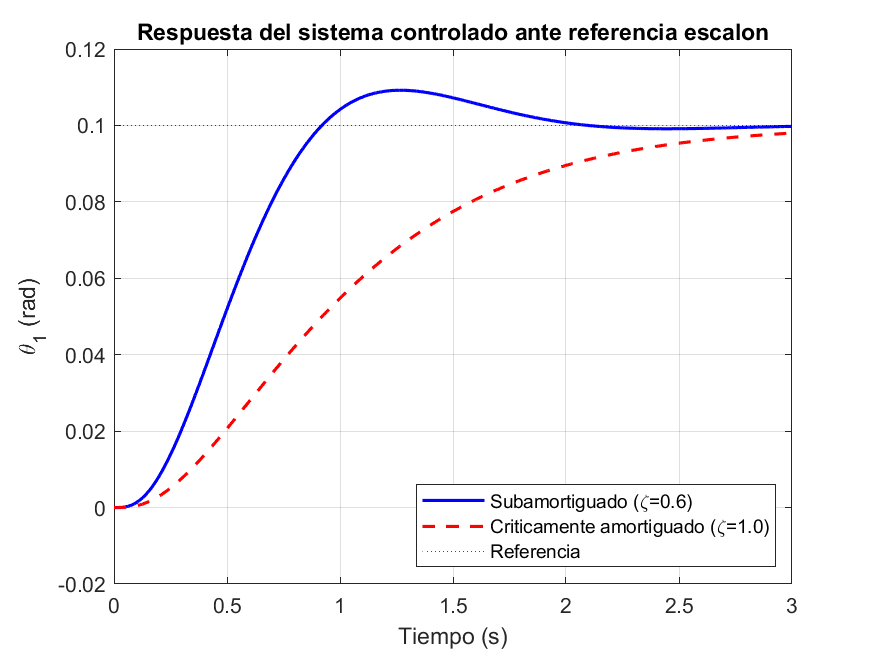
\includegraphics[width=0.95\linewidth]{simulations/figures/respuesta_controlador.png}
\caption{Respuesta del sistema controlado ante referencia escalón de 0.1 rad: diseño subamortiguado ($\zeta=0.6$) vs. críticamente amortiguado ($\zeta=1.0$).}
\label{fig:respuesta_controlador}
\end{figure}

Como se observa, el diseño con $\zeta=0.6$ presenta sobreimpulso (~9\,\%) y un tiempo de asentamiento cercano al valor de diseño de \SI{2}{s}, mientras que el diseño con $\zeta=1.0$ elimina el sobreimpulso a costa de una respuesta más lenta, consistente con la teoría de sistemas de segundo orden dominante.

\subsection{Observador de estados}

La Figura~\ref{fig:respuesta_observador} presenta la convergencia del error de estimación $e=\vec{x}-\hat{\vec{x}}$ para un error inicial $e_0=[0.05,\ 0.02,\ 0.01]^T$, usando las ganancias $L_{std}$ de la Sección~\ref{sec:observador}.

\begin{figure}[H]
\centering
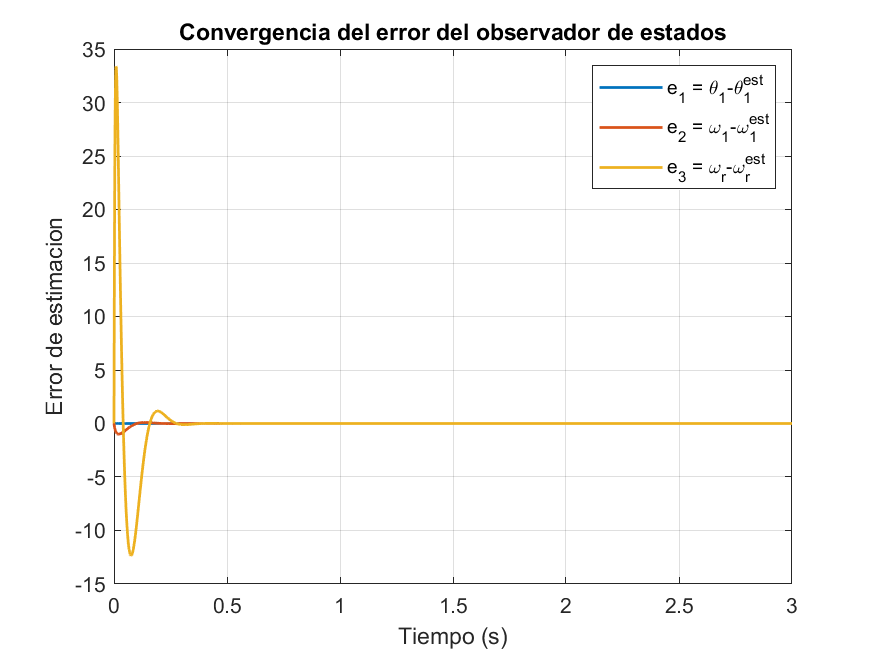
\includegraphics[width=0.95\linewidth]{simulations/figures/respuesta_observador.png}
\caption{Convergencia del error de estimación del observador de estados.}
\label{fig:respuesta_observador}
\end{figure}

El error converge a cero en aproximadamente \SI{0.4}{s}, un orden de magnitud más rápido que el tiempo de asentamiento del controlador (\SI{2}{s}), confirmando el criterio de diseño de un observador 10 veces más rápido. El pico transitorio observado en $e_3$ es característico de observadores de alta ganancia y no compromete la estabilidad, dado que los polos de $(A-LC)$ se ubicaron todos en el semiplano izquierdo.

\subsection{Servosistema}

La Figura~\ref{fig:respuesta_servo} muestra el seguimiento de la referencia $r=0.1\,\si{rad}$ por parte del servosistema completo (controlador + compensador integrante), correspondiente al diseño subamortiguado.

\begin{figure}[H]
\centering
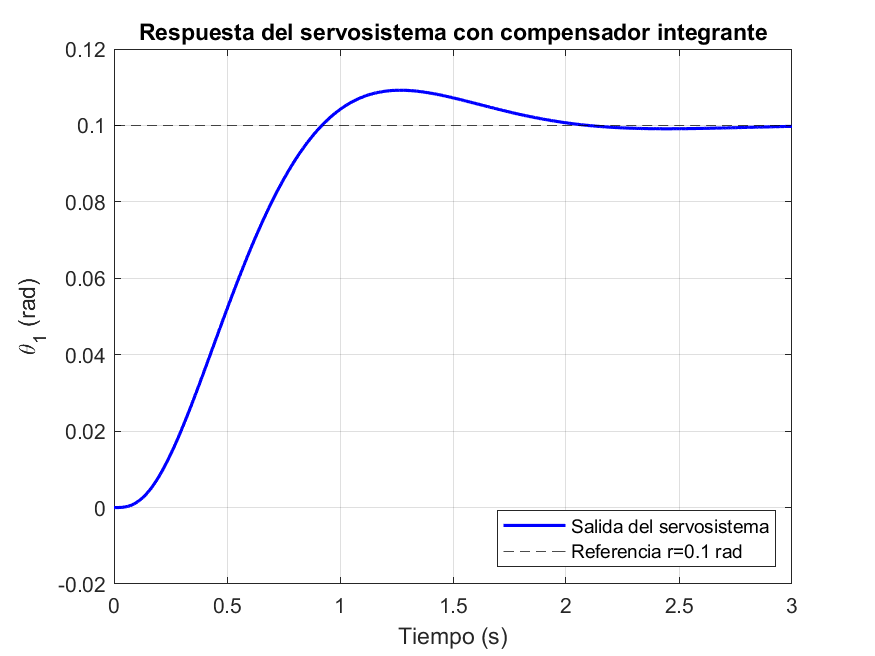
\includegraphics[width=0.95\linewidth]{simulations/figures/respuesta_servosistema.png}
\caption{Respuesta del servosistema con compensador integrante ante referencia escalón.}
\label{fig:respuesta_servo}
\end{figure}

El servosistema alcanza la referencia con error de estado estacionario nulo, validando la acción del compensador integrante incorporado en el diseño.

\section{Análisis de Resultados}

Los tres métodos de ubicación de polos evaluados --- asignación directa, compensación por matriz de pesos y método de Ackermann --- convergen a las mismas ganancias $K$, $K_i$ y $L$ para cada representación de estados, lo cual confirma que la ubicación de polos es única para un par $(A,B)$ controlable (o $(A,C)$ observable) dado un polinomio característico deseado, independientemente de la técnica algebraica empleada para calcularla. La diferencia observada en la magnitud numérica de las ganancias entre las representaciones estándar, canónica controlable y canónica observable se explica por el cambio de base introducido por las matrices de transformación $T_{cc}$ y $T_{co}$; el comportamiento entrada-salida del lazo cerrado, sin embargo, es idéntico en los tres casos, pues corresponde al mismo conjunto de polos deseados.

El controlador diseñado con $\zeta=0.6$ actúa como un filtro que prioriza velocidad de respuesta sobre sobreimpulso, mientras que el diseño con $\zeta=1.0$ prioriza ausencia de sobreimpulso a costa de un mayor tiempo de establecimiento; ambos resultados son consistentes con la teoría clásica de sistemas de segundo orden aplicada sobre los polos dominantes del sistema aumentado. La elevada ganancia del observador, necesaria para lograr una dinámica de error diez veces más rápida que el controlador, es coherente con la exigencia de estimar rápidamente estados no medibles ($\omega_1$, $\omega_r$) frente a un polo natural de planta relativamente rápido ($p_m=-24.93$).

\section{Conclusiones}

\begin{enumerate}
    \item Se obtuvo el modelo en espacio de estados del péndulo con rueda de reacción a partir de sus parámetros físicos, así como sus representaciones canónicas controlable y observable, verificando la controlabilidad y observabilidad completa del sistema en el punto de operación vertical.
    \item Se diseñaron controladores por retroalimentación de estados mediante tres metodologías equivalentes (asignación directa, matriz de pesos y Ackermann), obteniendo ganancias numéricamente idénticas entre métodos, lo que valida la unicidad de la solución de ubicación de polos para un sistema controlable.
    \item El observador de estados diseñado con dinámica diez veces más rápida que el controlador permitió una convergencia del error de estimación en aproximadamente una quinta parte del tiempo de asentamiento del controlador, validando el criterio de separación entre las dinámicas de observador y controlador.
    \item El servosistema con compensador integrante logró seguimiento de referencia con error de estado estacionario nulo, confirmando la efectividad del integrador añadido para plantas sin polo en el origen.
    \item La comparación entre los diseños subamortiguado y críticamente amortiguado evidenció el comportamiento del controlador por retroalimentación de estados como un filtro configurable, permitiendo ajustar el compromiso entre velocidad de respuesta y sobreimpulso mediante la selección del factor de amortiguamiento $\zeta$ de los polos dominantes.
\end{enumerate}

\section{Preguntas para la Discusión}

\begin{itemize}
    \item \textit{Pregunta 1: ¿El controlador por retroalimentación de estados puede representar a un filtro de qué tipo?} La ley $u=-K\vec{x}$ ubica los polos en lazo cerrado, por lo que el sistema resultante se comporta como un filtro pasa-bajas de segundo orden dominante, cuyo ancho de banda y factor de amortiguamiento son directamente configurables mediante la elección de los polos deseados, como se evidenció al comparar los diseños con $\zeta=0.6$ y $\zeta=1.0$.
    \item \textit{Pregunta 2: Hay diversas representaciones de los sistemas en espacio de estados, ¿el controlador para todas estas representaciones es el mismo?} No en magnitud numérica, pero sí en efecto: cada representación (estándar, FCC, FCO) requiere una matriz $K$ distinta, relacionada mediante las transformaciones de similitud $T_{cc}$, $T_{co}$, pero todas ubican exactamente los mismos polos en lazo cerrado y producen la misma respuesta entrada-salida.
    \item \textit{Pregunta 3: ¿Para implementar un control por retroalimentación de estados en un sistema no lineal sería posible sin observadores de estado?} Solo sería posible si todos los estados del modelo linealizado son físicamente medibles con sensores; en el péndulo con rueda de reacción, $\omega_1$ y $\omega_r$ no siempre son medibles directamente, por lo que en la práctica se requiere un observador.
    \item \textit{Pregunta 4: De ser afirmativa la respuesta anterior, ¿qué condiciones debería tener esta implementación?} Se requeriría instrumentación completa (sensores de posición y velocidad angular en barra y rueda) con ancho de banda y resolución suficientes, y el sistema debería permanecer dentro de la región de validez de la linealización utilizada para el diseño de $K$.
\end{itemize}

\bibliographystyle{IEEEtran}
\begin{thebibliography}{99}

\bibitem{ogata_discreto}
K. Ogata, \textit{Sistemas de Control en Tiempo Discreto}, Prentice Hall Internacional, 1996.

\bibitem{kuo_digital}
B. C. Kuo, \textit{Digital Control System}, Rinehart and Winston, 1996.

\bibitem{unam_tutorial}
F. d. l. l. UNaM, ``Tutoriales de Control con MATLAB,'' Regents of University of Michigan, 18 Agosto 1997. [En línea]. Available: http://www.ib.cnea.gov.ar/~instyctl/Tutorial\_Matlab\_esp/index.html. [Último acceso: 22 Enero 2013].

\bibitem{franklin_digital}
G. F. Franklin, J. D. Powell y M. L. Workman, \textit{Digital Control of Dynamic Systems}, Prentice Hall, 1998.

\bibitem{phillips_digital}
C. Phillips, \textit{Digital Control System Analysis and Design}, Prentice Hall.

\bibitem{constantine_digital}
H. Constantine y G. B. Lamont, \textit{Digital Control Systems}, McGraw-Hill Companies.

\end{thebibliography}

\section*{Anexo: Código MATLAB}

El siguiente listado corresponde al script \texttt{simulation.m}, empleado para obtener las matrices del sistema, las formas canónicas y las ganancias del controlador y del observador presentadas en las Secciones~\ref{sec:modelo}--\ref{sec:servo}.

\lstinputlisting[language=Matlab, caption={Script de diseño: modelo, formas canónicas, controlador y observador}, label={lst:simulation_m}]{simulations/simulation.m}

El siguiente listado corresponde al script \texttt{post\_process.m}, empleado para simular la respuesta en lazo cerrado y generar las Figuras~\ref{fig:respuesta_controlador}--\ref{fig:respuesta_servo}.

\lstinputlisting[language=Matlab, caption={Script de post-procesamiento: respuestas de controlador, observador y servosistema}, label={lst:post_process_m}]{simulations/post_process.m}

\section*{Anexo: Modelado del Sistema}

\begin{figure*}[t]
\centering
\imgplaceholder{8cm}{Espacio reservado -- Foto 1: Modelado del sistema (péndulo con rueda de reacción)}
\caption{Modelado del sistema péndulo con rueda de reacción (parte 1).}
\label{fig:modelado_1}
\end{figure*}

\begin{figure*}[t]
\centering
\imgplaceholder{8cm}{Espacio reservado -- Foto 2: Modelado del sistema (péndulo con rueda de reacción)}
\caption{Modelado del sistema péndulo con rueda de reacción (parte 2).}
\label{fig:modelado_2}
\end{figure*}

\end{document}

